\chapter{Détermination du diamètre optimal des intervalles à considérer pour l'estimation de la régularité locale }
\minitoc%

\section{Introduction et Objectifs de la simulation}

\section{Simulation de données $\operatorname{FAR}(1)$ Localement Hölderiennes}

La fonction $H : t \mapsto H_t$ qui a été choisie est la suivante :

$$
H^{[0.4, 0.8, 5, 0.5]}_{\textsf{logistic}} : \begin{array}{ccc}
    [0,1] & \longrightarrow & [0.4, 0.8]
    \\
    t & \longmapsto & 0.4 + \frac{(0.8 - 0.4)}{1 + e^{-5(t - 0.5)}}
\end{array}
$$

$$\forall t \quad L_t = 1$$

$$
\mu : \begin{array}{ccc}
    [0,1] & \longrightarrow & \mathbb R
    \\
    t & \longmapsto & 4 \cdot \sin\bigl( \frac 3 2 \pi \cdot t \bigr)
\end{array}
$$

$$
\vec t = \begin{bmatrix} 0.3 \\ 0.4 \\ 0.5 \\ 0.6 \\ 0.7 \\ 0.8 \end{bmatrix}
\quad\quad
H(\, \vec t \,) = 
\begin{bmatrix}
    0.51 \\ 0.55 \\ 0.6 \\ 0.65 \\ 0.69 \\ 0.73
\end{bmatrix}
$$

$$
\beta : \, \begin{array}{ccc}
    [0,1]^2 & \longrightarrow & \mathbb R
    \\
    (t,s) & \longmapsto & \frac 9 4 t\sqrt{ s(1-s) }
\end{array}
$$

$$
\vec N = [ 100, 200, 300, 400]
$$

$$
\vec \Delta = [ 0.01 \cdots (0.01 + k\cdot0.01)\cdots 0.2 ]_{k \in 0:30}
$$

En résumé :

\begin{table}[H]
    \centering
    \begin{tabular}{l|l|ll|l|}
    \cline{2-5}
    \textbf{}                                                         & \textbf{nombre de valeurs testées} & \multicolumn{1}{l|}{\textbf{de}} & \textbf{jusqu'à}         & \textbf{valeur}          \\ \hline
    \multicolumn{1}{|l|}{\textit{\textbf{$\Delta$}}}                  & $30$                               & $0.01$                        & $0.2$                   & \cellcolor[HTML]{C0C0C0} \\
    \multicolumn{1}{|l|}{\textit{\textbf{$\lambda$}}}                 & $30$                               & $30$                             & $480$                    & \cellcolor[HTML]{C0C0C0} \\
    \multicolumn{1}{|l|}{\textit{\textbf{$N$}}}                       & $4$                                & $100$                            & $400$                    & \cellcolor[HTML]{C0C0C0} \\
    \multicolumn{1}{|l|}{\textit{\textbf{fonction de Hurst ($H_t$)}}} & $2$                                & logistique                       & escalier                 & \cellcolor[HTML]{C0C0C0} \\
    \multicolumn{1}{|l|}{\textit{\textbf{nb simulations MC}}}         & \cellcolor[HTML]{C0C0C0}           & \cellcolor[HTML]{C0C0C0}         & \cellcolor[HTML]{C0C0C0} & $200$                    \\ \hline
    \end{tabular}
    \caption{Hyper-paramètres de la simulation Monte-Carlo}
    \label{tab:hyperparam-mc}
    \end{table}


\section{Prélissage des données simulées}




\section{Qualité de l'estimation des incréments quadratiques moyens}

\newcommand{\thetaA}{\Theta_{1 \rightarrow \overset{3}{\underset {2}{}}}}
\newcommand{\cindexA}{_{1 \rightarrow \overset{3}{\underset {2}{}}}}
\newcommand{\thetaB}{\Theta_{\overset 1{\underset{2}{ }} \rightarrow3}}
\newcommand{\cindexB}{_{\overset 1{\underset{2}{ }} \rightarrow3}}
\newcommand{\thetaC}{\Theta_{1 \rightarrow 2 \rightarrow 3}}
\newcommand{\cindexC}{_{1 \rightarrow 2 \rightarrow 3}}
\newcommand{\notequiv}{\overset {\textsf{\faTimes}} \iff}
\newcommand{\yesequiv}{\overset {\textsf{\faCheck}} \iff}

Il y a différentes manières de définir les paramètres de régularité $\hat H_t$ et $\hat L_t$. En effet il est possible de définir $\hat H_t$ en utilisant $\hat \theta (t_1, t_2)$ mais aussi en utilisant $\hat \theta (t_2, t_3)$ ($\theta(t_1, t_3)$ est forcément utilisé\footnote{$\hat H_t$ ne serait même pas bien défini pour le couple $\theta(t_1, t_2)$, $\theta(t_2, t_3)$}). De même pour $\hat L_t$. On peut donc se demander quels sont les meilleurs $\theta(u,v)$ avec $u,v \in \{t_1, t_2, t_3\}$ à utiliser pour obtenir la meilleure estimation de $H_t$ et $L_t$ ainsi que leur $\Delta$ optimal associé pour l'estimation de ces paramètres.

Le problème est que le proxy $\theta$ est défini comme une espérance, et donc n'est pas observable. On ne peut donc pas directement comparer $\hat \theta(u,v) = \sum_i|\widehat X_i(u) - \widehat X_i(v)|^2$ et $\theta(u,v) = \esperanceloi X { |X(u) - X(v)|^2 }$, à moins d'avoir fait le calcul de l'expression explicite en connaissant la loi du processus initial. 

On peut cependant comparer $\hat \theta(u,v)$ et $\widetilde \theta(u,v) = \frac 1 N \sum_i |X_i(u) - X_i(v)|^2$ qui est un estimateur de $\theta(u,v)$, et que l'on obtient aisément avec la simulation. On peut ainsi déterminer pour quelle valeur de $\Delta$ et quel couple $(u,v)$ on dispose de la meilleur estimation du $\tilde \theta$, qui est entre-autre le meilleur estimateur que l'on pourrait espérer de $\theta$.


Le meilleur couple (au sens donné dans cette section) est pris comme étant les deux $\hat \theta(u,v)$ réalisant les risques minimaux par rapport au $\tilde \theta$ sur les 3 couples $(u,v)$ possibles. 

    \begin{table}[H]
        \centering
        \begin{tabular}{l|ll|}
            \cline{2-3}
            & $\lambda < 120$                                                                                            & $\lambda \geq 120$                                                                 \\ \hline
            \multicolumn{1}{|l|}{$H_t < 0.6$}    & \multicolumn{1}{l|}{\begin{tabular}[c]{@{}l@{}}$\thetaC$\\ \\ \\ $\Delta^- \rightarrow 0.01$\end{tabular}} & \begin{tabular}[c]{@{}l@{}}$\thetaA$\\ \\ $\Delta^+ \rightarrow 0.2$\end{tabular}  \\ \cline{2-3} 
            \multicolumn{1}{|l|}{$H_t \geq 0.6$} & \multicolumn{1}{l|}{\begin{tabular}[c]{@{}l@{}}$\thetaA$\\ \\ $\Delta^- \rightarrow 0.2$\end{tabular}}     & \begin{tabular}[c]{@{}l@{}}$\thetaC$\\ \\ $\Delta^+ \rightarrow 0.01$\end{tabular} \\ \hline
        \end{tabular}
        \caption{Tableau récapitulatif des $\Theta$ optimaux : Risque individuel sur $\tilde \theta(u,v)$}
        \label{tab:recap_theta_single}
    \end{table}



\section{Qualité de l'estimation de la régularité locale}

Les simulations de Monte Carlo permettent d'avoir accès directement à la véritable régularité de la courbe en chaque point. Nous allons dans l'étude du comportement du $\Delta$ essayer de tirer profit de cet avantage que ne possède pas le praticien qui utilise des données réelles.


\begin{table}[H]
    \centering
    \begin{tabular}{l|ll|}
    \cline{2-3}
                                          & $\lambda < 120$                                                                                                                                                                                                                                                                                    & $\lambda \geq 120$                                                                                                                                                                         \\ \hline
    \multicolumn{1}{|l|}{$H_t \leq 0.65$} & \multicolumn{1}{l|}{\begin{tabular}[c]{@{}l@{}}$\yesequiv \mathcal R$\\ $\yesequiv \Delta^*$\\ $\Delta^- \downarrow 0.01$\end{tabular}}                                                                                                                                             & \begin{tabular}[c]{@{}l@{}}$\simeq \yesequiv \mathcal R$\\ $\notequiv \Delta^*$\\ $\Delta^+ \rightarrow [\leq 0.6] 0.1/0.2 [\geq 0.6]$\end{tabular}                            \\ \cline{2-3} 
    \multicolumn{1}{|l|}{$H_t > 0.65$}    & \multicolumn{1}{l|}{\begin{tabular}[c]{@{}l@{}}$\yesequiv \mathcal R$\\ $\notequiv \Delta^*$\\ \faExclamationTriangle $H=0.7 : \Delta^- = 0.02$\\ \faExclamationTriangle $H = 0.73 : \Delta^- = 0.2$\end{tabular}} & \begin{tabular}[c]{@{}l@{}}$\thetaA$\\ \faExclamationTriangle $H=0.7 : \Delta^+ = 0.02$\\ \faExclamationTriangle $H = 0.73 : \Delta^+ = 0.2$\end{tabular} \\ \hline
    \end{tabular}
    \caption{Tableau récapitulatif des $\Delta$ optimaux : Risque sur $H_t$}
    \label{tab:recap_delta_H}
    \end{table}

\section{Qualité de l'estimation des couples d'incréments utilisés dans l'estimation de la régularité}


\info{
    on rappelle les notations suivantes :

    \begin{itemize}
        \item vrai : $\theta = \mathds E \bigl[ \, f(X) \, \bigr]$
        \item intangible : $\widetilde \theta = \frac 1 N \sum_i f(X_i)$
        \item observable : $\hat \theta = \frac 1 N \sum_i f(\widehat X_i)$ 
    \end{itemize}
}

L'estimateur du paramètre de régularité $H_t$ est donné par :

$$\hat H_t = \frac{ \log \hat \theta(t_1, t_3) - \log \hat \theta(t_1, t_2) }{2 \log 2}$$

ou bien encore :

$$\hat H_t = \frac{ \log \hat \theta(t_1, t_3) - \log \hat \theta(t_2, t_3) }{2 \log 2}$$


autrement dit :

en posant $\thetaA = \begin{bmatrix} \theta(t_1, t_3) \\ \theta(t_1, t_2) \end{bmatrix}$ et $\thetaB = \begin{bmatrix} \theta(t_1, t_3) \\ \theta(t_2, t_3) \end{bmatrix}$

$$
\hat H_t : \Theta \longmapsto \frac{ \log \Theta_1 - \log \Theta_2 }{2 \log 2}
$$

C'est pourquoi, étant donné que le meilleur estimateur que l'on puisse espérer soit $\bigl(\hat H_t( \tilde \thetaA)$ ou $\hat H_t( \tilde \thetaB)\bigr)$, on va s'intéresser désormais à l'estimation conjointe des deux $\theta(u,v)$ utilisés dans l'estimation de $H_t$ comme critère de sélection du diamètre $\Delta$.

\begin{figure}[H]
    \centering
    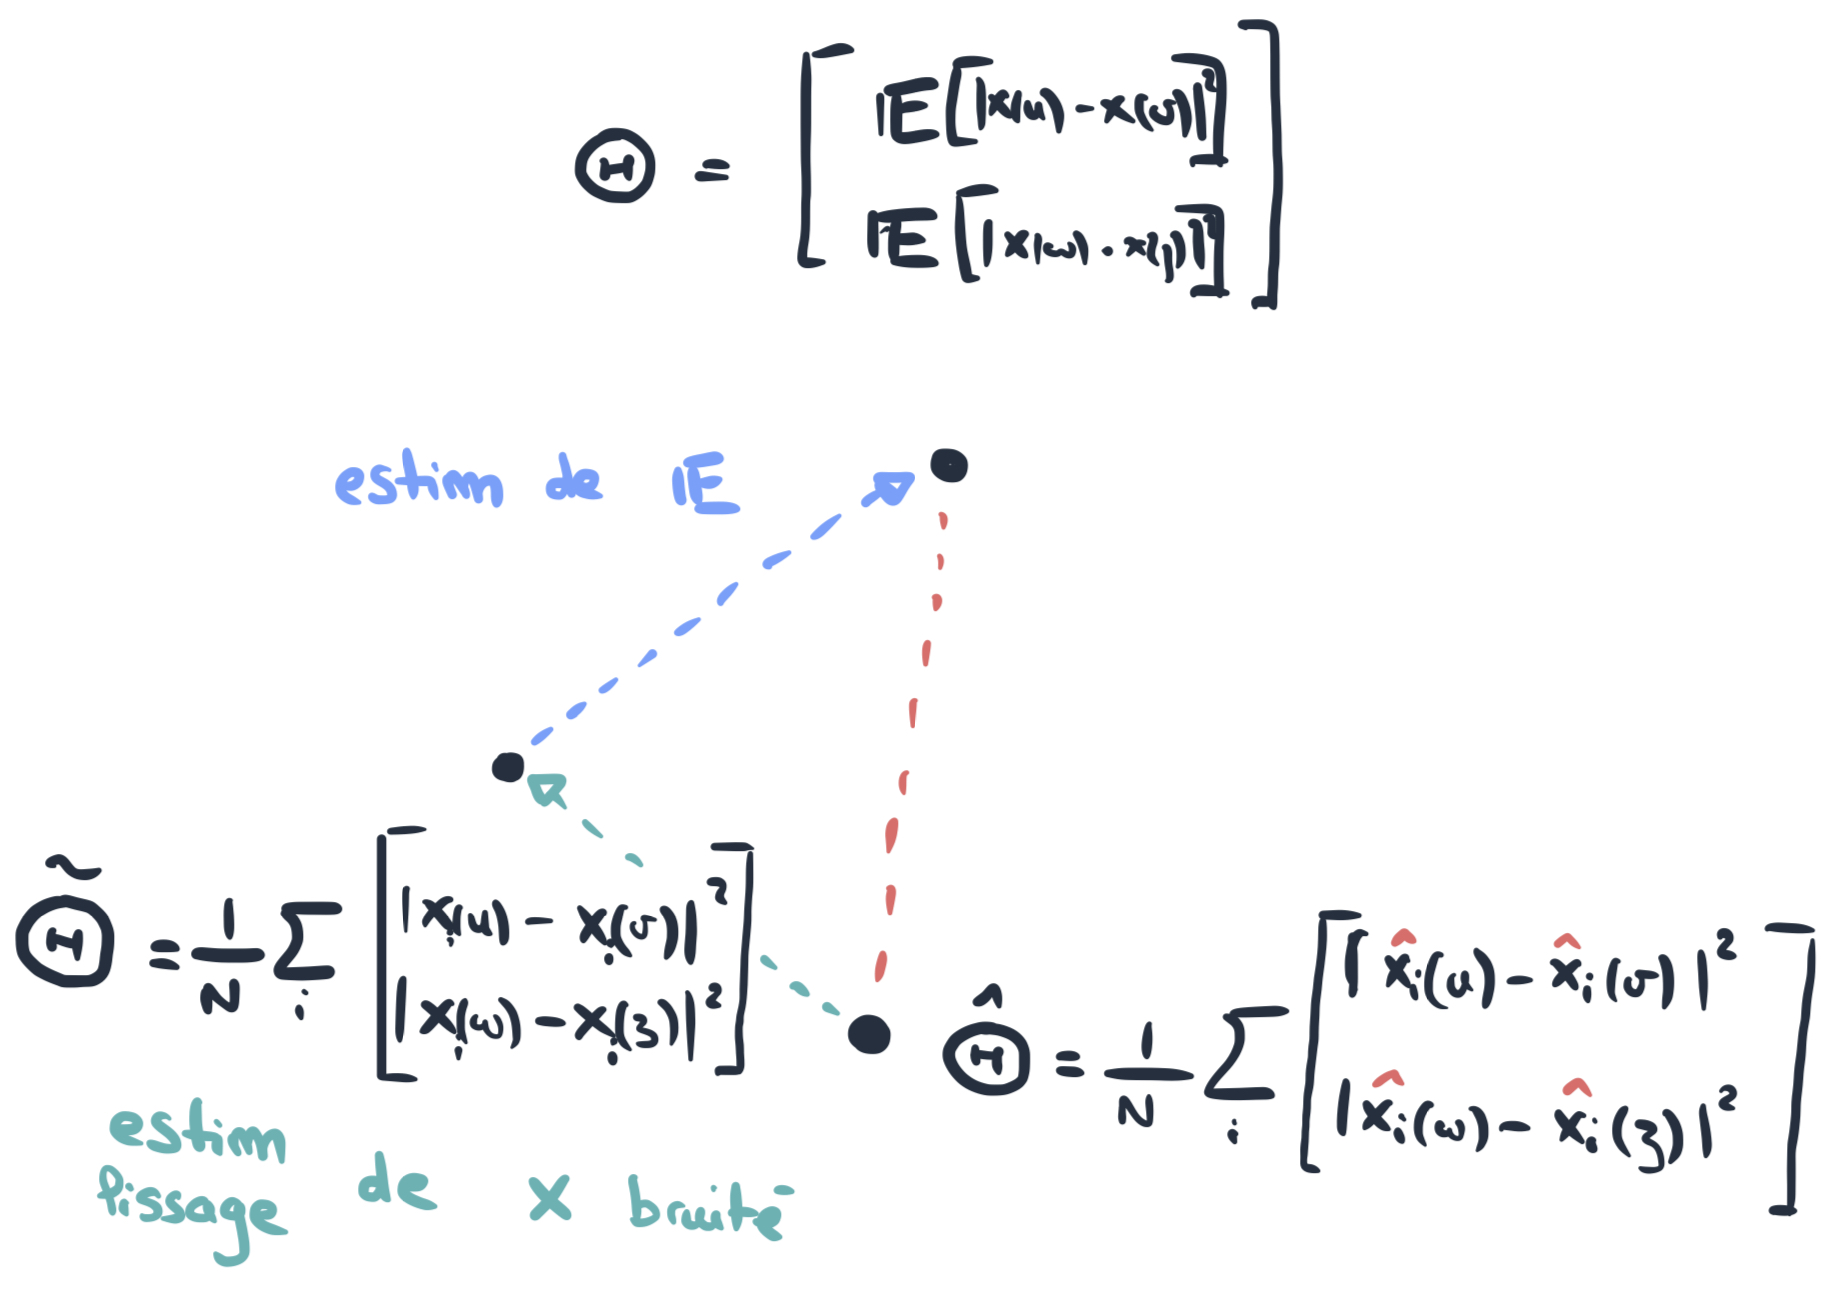
\includegraphics[width=0.7\textwidth]{Images/sketches/theta_biais.jpg}
    \caption{title}
    \label{fig:sketch_theta_biais}
\end{figure}


Pour cela on considère la distance euclidienne usuelle pour des vecteurs de $\R 2$

$$R(\Theta, \Delta) = \distnorme 2 {\widehat \Theta(\Delta)} {\widetilde \Theta(\Delta)}$$

et on nomme $R\cindexA = R( \thetaA , \, \cdot \, )$ et $R\cindexB = R( \thetaB, \, \cdot \, )$

\begin{table}[H]
    \centering
    \begin{tabular}{l|ll|}
    \cline{2-3}
                                         & $\lambda < 120$                                                                                                                                                                                                                                     & $\lambda \geq 120$                                                                             \\ \hline
    \multicolumn{1}{|l|}{$H_t < 0.6$}    & \multicolumn{1}{l|}{\begin{tabular}[c]{@{}l@{}}$\yesequiv \mathcal R, \Delta^*$\\ $\Delta^*_- = 0.01$\end{tabular}}                                                                                                                                 & \begin{tabular}[c]{@{}l@{}}$\thetaB$\\ $\Delta^*_+ = 0.2$\end{tabular}                         \\ \cline{2-3} 
    \multicolumn{1}{|l|}{$H_t \geq 0.6$} & \multicolumn{1}{l|}{\begin{tabular}[c]{@{}l@{}}$\thetaB$\\ $\Delta^*_- = 0.2$\\ \\\faExclamationTriangle $H=0.7 : \Delta^- = 0.01 \oplus \yeqequiv \mathcal R$\\ \\\faExclamationTriangle $H=0.8 : \thetaA$\end{tabular}} & \begin{tabular}[c]{@{}l@{}}$\yesequiv \mathcal R, \Delta^*$\\ $\Delta^*_+ = 0.01$\end{tabular} \\ \hline
    \end{tabular}
    \label{tab:recap_delta_eucl}
    \caption{Tableau récapitulatif des $\Delta$ optimaux : Risque euclidien sur $\tilde \Theta$}
    \end{table}

\section{Détermination d'un critère de choix du diamètre $\Delta$ des intervalles à considérer pour l'estimation de la régularité locale}


Maintenant que l'on a déterminé que l'on souhaite travailler sur un les couples $\thetaB = \begin{bmatrix} \theta(t_1, t_3) \\ \theta(t_2, t_3) \end{bmatrix}$ et $\thetaA = \begin{bmatrix} \theta(t_1, t_3) \\ \theta(t_1, t_2) \end{bmatrix}$, il nous faut déterminer un critère pour déterminer quel couple est plus judicieux pour la méilleure estimation en pratique des paramètres de régularité locale.

L'heuristique est la suivante : dans nos simulations, on a le luxe de pouvoir faire 200 simulations de monte carlo et obtenir le $\Delta^*$ le plus proche du $\Delta$ optimal pour estimer la régularité. Dans la pratique, obtenir un tel $\Delta$ optimal n'est pas réaliste, on se trouvera soit un peu en dessous, soit un peu au dessus. L'idée est donc de favoriser le couple de $\theta(u,v)$ qui possède le plus grand plateau autour du $\Delta^*$ pour le risque quadratique \emph{si l'écart de risque quadratique entre les deux couples n'est pas trop important}. Si l'un est beaucoup plus performant que l'autre, on choisira le plus performant. Mais si la performance des deux est à peu près équivalente, autant sélectionner celui qui dans la pratique (sans avoir 200 réplications indépendantes) nous donnera le plus de flexibilité sur l'erreur commise en sélectionnant un $\Delta$ autour du $\Delta^*$ dû à la fluctuation statistique.

\subsection{Détermination d'un seuil pour l'équivalence de risque quadratique}

Il nous faut maintenant déterminer ce que l'on considère comme étant deux risques "équivalents". Pour cela on va déterminer pour différentes valeurs du véritable $H$ le seuil $\varepsilon$ sur le risque tel que $R\cindexA(\Delta + \delta) + \varepsilon$ induit une erreur d'au maximum $10$\% sur le H estimé. On viendra ensuite déterminer les $\delta$ qui en moyenne correspondent à ce seuil $\varepsilon$ pour les différentes valeurs de $H$.

\subsection{Détermination du meilleur couple à risque \og équivalent \fg}

\subsubsection{en utilisant les pentes}


Une méthode possible serait de définir la pente à gauche et la pente à droite de la façon suivante : 

$$a_g : \Delta, \delta \mapsto \frac{R(\Delta) - R(\Delta - \delta)}{\delta}$$
$$a_d : \Delta, \delta \mapsto \frac{R(\Delta + \delta) - R(\Delta)}{\delta}$$

On peut définir les pénalisations suivantes pour déterminer le meilleur couple à risque équivalent en terme de plateau, en pénalisant les larges différence entre la pente à gauche et à droite :

$$m_q(\Delta, \delta) = \frac{a_g^2(\Delta, \delta) + a_d^2(\Delta, \delta)}{2}$$


\subsubsection{en utilisant les valeurs de risque}
une autre méthode est de regarder :

$$R_2(\Delta^*_2) \geq R_1(\Delta^*_1)$$

$$dR = \bigl\vert R_1(\Delta^*_1) - R_2(\Delta^*_2) \bigr\vert$$

on compare désormais les valeurs de :

$$r_g^{[2]} = R_2(\Delta^*_2 - \delta) - dR$$ 
$$r_d^{[2]} = R_2(\Delta^*_2 + \delta) - dR$$ 

aux valeurs

$$r_g^{[1]} = R_1(\Delta^*_1 - \delta)$$ 
$$r_d^{[1]} = R_1(\Delta^*_1 + \delta)$$

avec le critère de sélection suivant :

$$\argmin \bigl( \frac{r_g^{[1]} + r_d^{[1]}}{2}, \frac{r_g^{[2]} + r_d^{[2]}}{2}  \bigr)$$

Pour pénaliser les solutions où la pente à gauche est très différente de la pente à droite en magnitude, on peut considérer d'élever $r_g$ et $r_d$ au carré.

$$\argmin \bigl( \frac{(r_g^{[1]})^2 + (r_d^{[1]})^2}{2}, \frac{(r_g^{[2]})^2 + (r_d^{[2]})^2}{2}  \bigr)$$

\subsubsection{résultat}